\documentclass[12pt]{article}
\usepackage[utf8]{inputenc}
\usepackage[french]{babel}
\usepackage{amsmath,amsthm,amsfonts,amssymb}
\usepackage{lmodern}
\usepackage[top=2.4cm,bottom=2.4cm,left=2cm,right=2cm]{geometry}
\usepackage{hyperref}
\usepackage{multicol}
\usepackage{enumitem}
\usepackage{listings}
\usepackage[dvipsnames]{xcolor}
\usepackage{tikz}

%\date{}
\title{{\bf  Génie logiciel} \\
	Notes du cours de 16/12 P \no 2  \\
	{\small L3 Informatique appliquée 2022-2023} \\
	{\it \small MABROUK Fayez}}
\begin{document}
	\maketitle
	\newpage
	\section{Documentation}
	\subsection{Introduction}
	\begin{itemize}
		\item[* ] Un bon logiciel doit s'accompagner d'une bonne documentation
		\item[* ] Définition : l'ensemble des documents écrits et du matériel (par exemple, figures, diagrammes)
		qui accompagne les logiciels informatiques
		\item[* ] Partie essentielle de l'ingénierie logicielle
		\item[* ] Objectif principal de la documentation : communication durable avec :\\
		\begin{itemize}
			\item[* ] Les parties prenantes
			\item[* ] les équipes de développement
			\item[* ] les utilisateurs
		\end{itemize}
	\end{itemize}
\subsection{Types de documents - Contractuels}
\begin{itemize}
	\item[* ] Cahier des charges (Specification) : décrit les exigences et les contraintes du projet.
	\item[* ] Contrat
	\item[* ] Convention : document contractuel suivant une forme convenue
	\item[* ] Réception : formalisation de la fin d'un projet
\end{itemize}
\subsection{Types de documents - Documents d'appui}
\begin{itemize}
	\item[* ] Présentation du logiciel : présentation générale du logiciel, sans
	détails.
	\item[* ] Manuel d'utilisation : décrit les fonctionnalités du logiciel et la manière de les utiliser.
	\item[* ] Manuel d'installation : décrit les procédures d'installation du manuel.
	\item[* ] Manuel d'exploitation : procédures de dépannage, de maintenance et de mises à jour
\end{itemize}
\subsection{Types de documents - Gestion de projet}
\begin{itemize}
	\item[* ] Plan de développement : définit les procédures pour réaliser le projet
	\item[* ] Conception : décrit le résultat de la phase de conception.
	\item[* ] Rapports de projet : rapports intermédiaires pour documenter le processus de développement.
	\item[* ] Feedback : vers la fin d'un projet, qu'avons-nous appris ? Qu'est-ce qui peut être réutilisé ?
\end{itemize}
\subsection{Types de documents - Qualité}
\begin{itemize}
	\item[* ] Plan d'assurance qualité : s'il est suivi, il garantit que le produit fini répond à
	tous les critères de qualité prédéfinis
	\item[* ] Plan d'audit interne : définit la fréquence et les procédures des audits internes.
	\item[* ] Plan d'évaluation : à la fin de chaque phase, vérifier que les objectifs initiaux sont
	atteints.
	\item[* ] Plan de test : à la fin du projet, valider que les objectifs initiaux sont atteints.
\end{itemize}
\subsection{Rédaction d'un document - Structure générale}
\begin{itemize}
	\item[* ] Identification du document :
	\begin{itemize}
		\item[* ] Nom du document
		\item[* ] Nom du projet
		\item[* ] Nom des auteurs / institutions
		\item[* ] Date du document
		\item[* ] Version du document
		
	\end{itemize}
\item[* ] Qualité du document :
\begin{itemize}
	\item[* ] Informations sur la vérification
	\item[* ] Informations sur la validation
	\item[* ] Informations sur la confidentialité
	\item[* ] Mots clés
\end{itemize}
\item[* ] Plan d'ensemble
\item[* ] Liste des figures
\item[* ] Liste des tableaux
\item[* ] Introduction :
\begin{itemize}
	\item[* ] Contexte
	\item[* ] Objectifs du document
	\item[* ] Résumé
	\item[* ] Rappel sur les notions nécessaires
	\item[* ] Comment lire ce document : guide de lecture pour chaque catégorie de lecteur
\end{itemize}
\item[* ] Le contenu spécifique du document
\item[* ] Lexique
\item[* ] Références
\item[* ] Index
\end{itemize}
\subsection{Cahier des charges}
\newpage
	\begin{figure}[!hbtp]
	\centering
	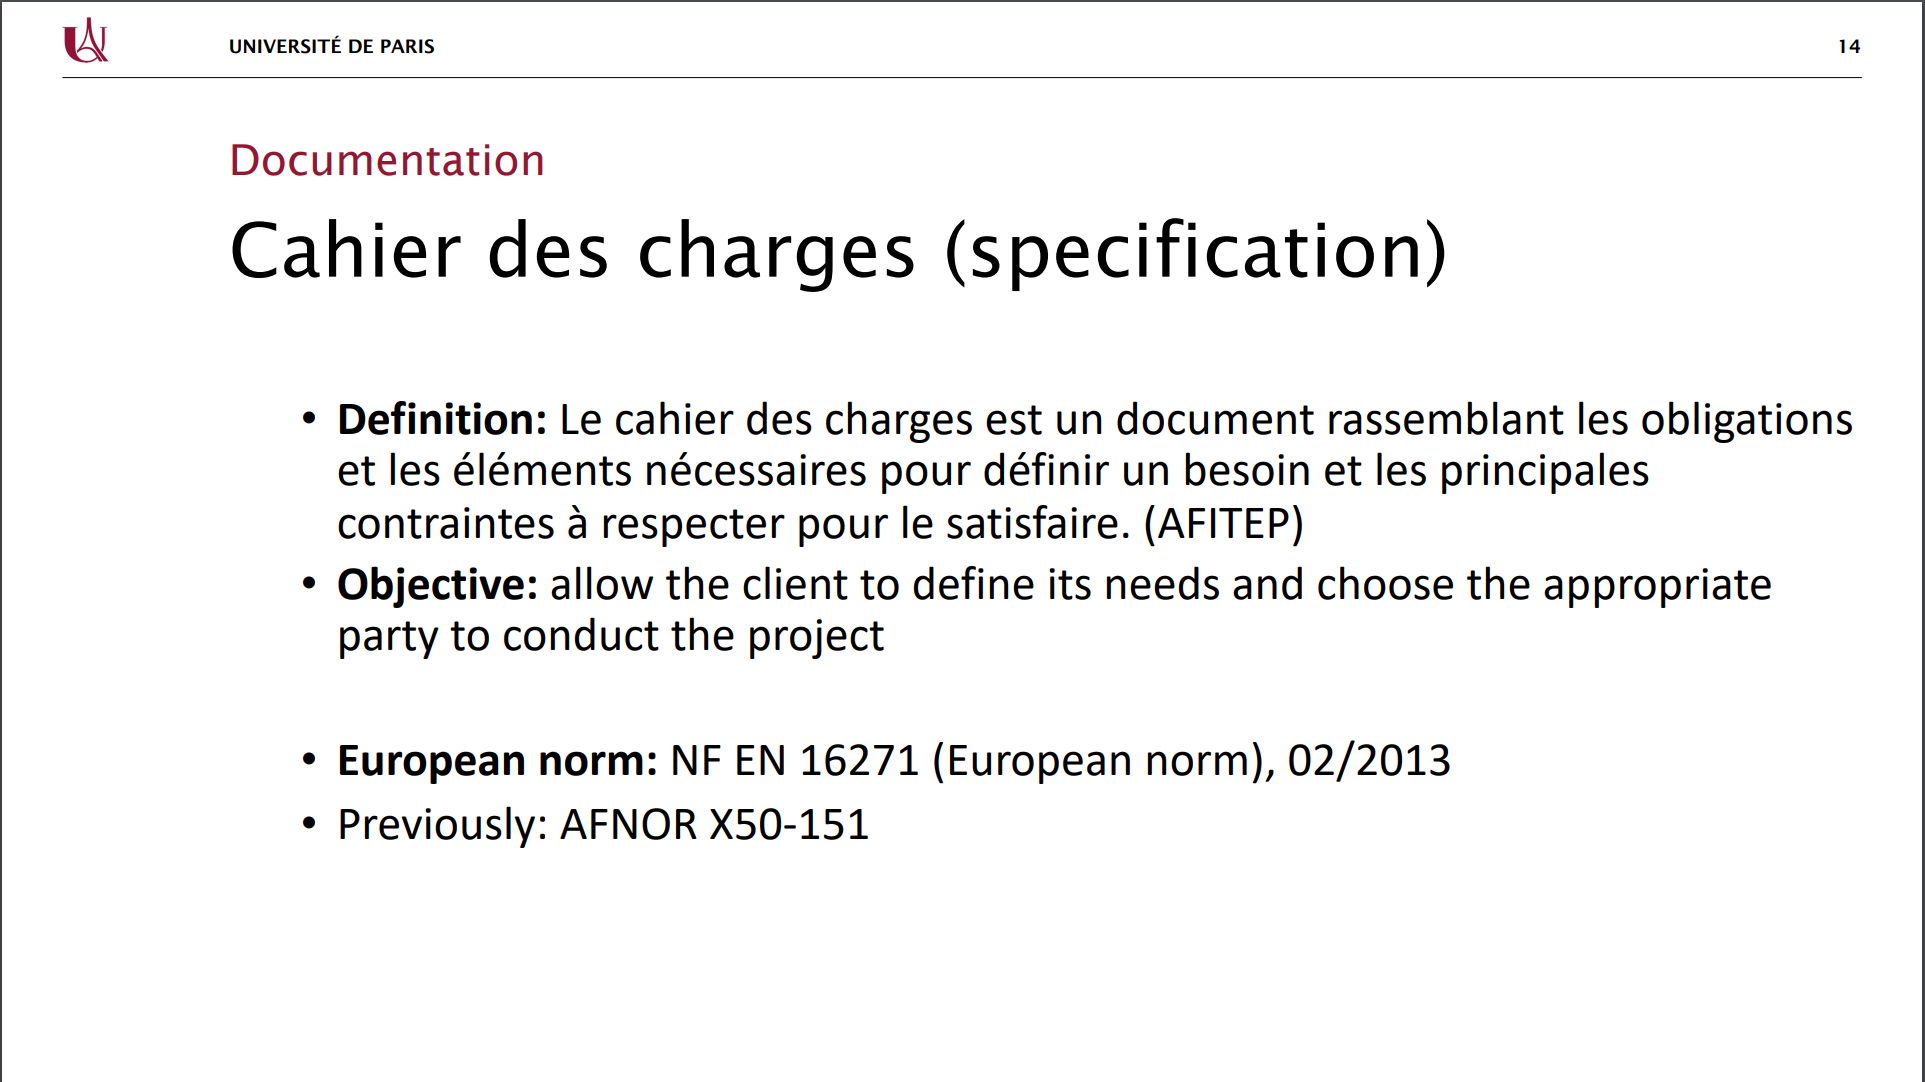
\includegraphics[scale=0.75]{Capture.PNG}
	%\caption{Légende de l'image}
\end{figure}
	\begin{figure}[!hbtp]
	\centering
	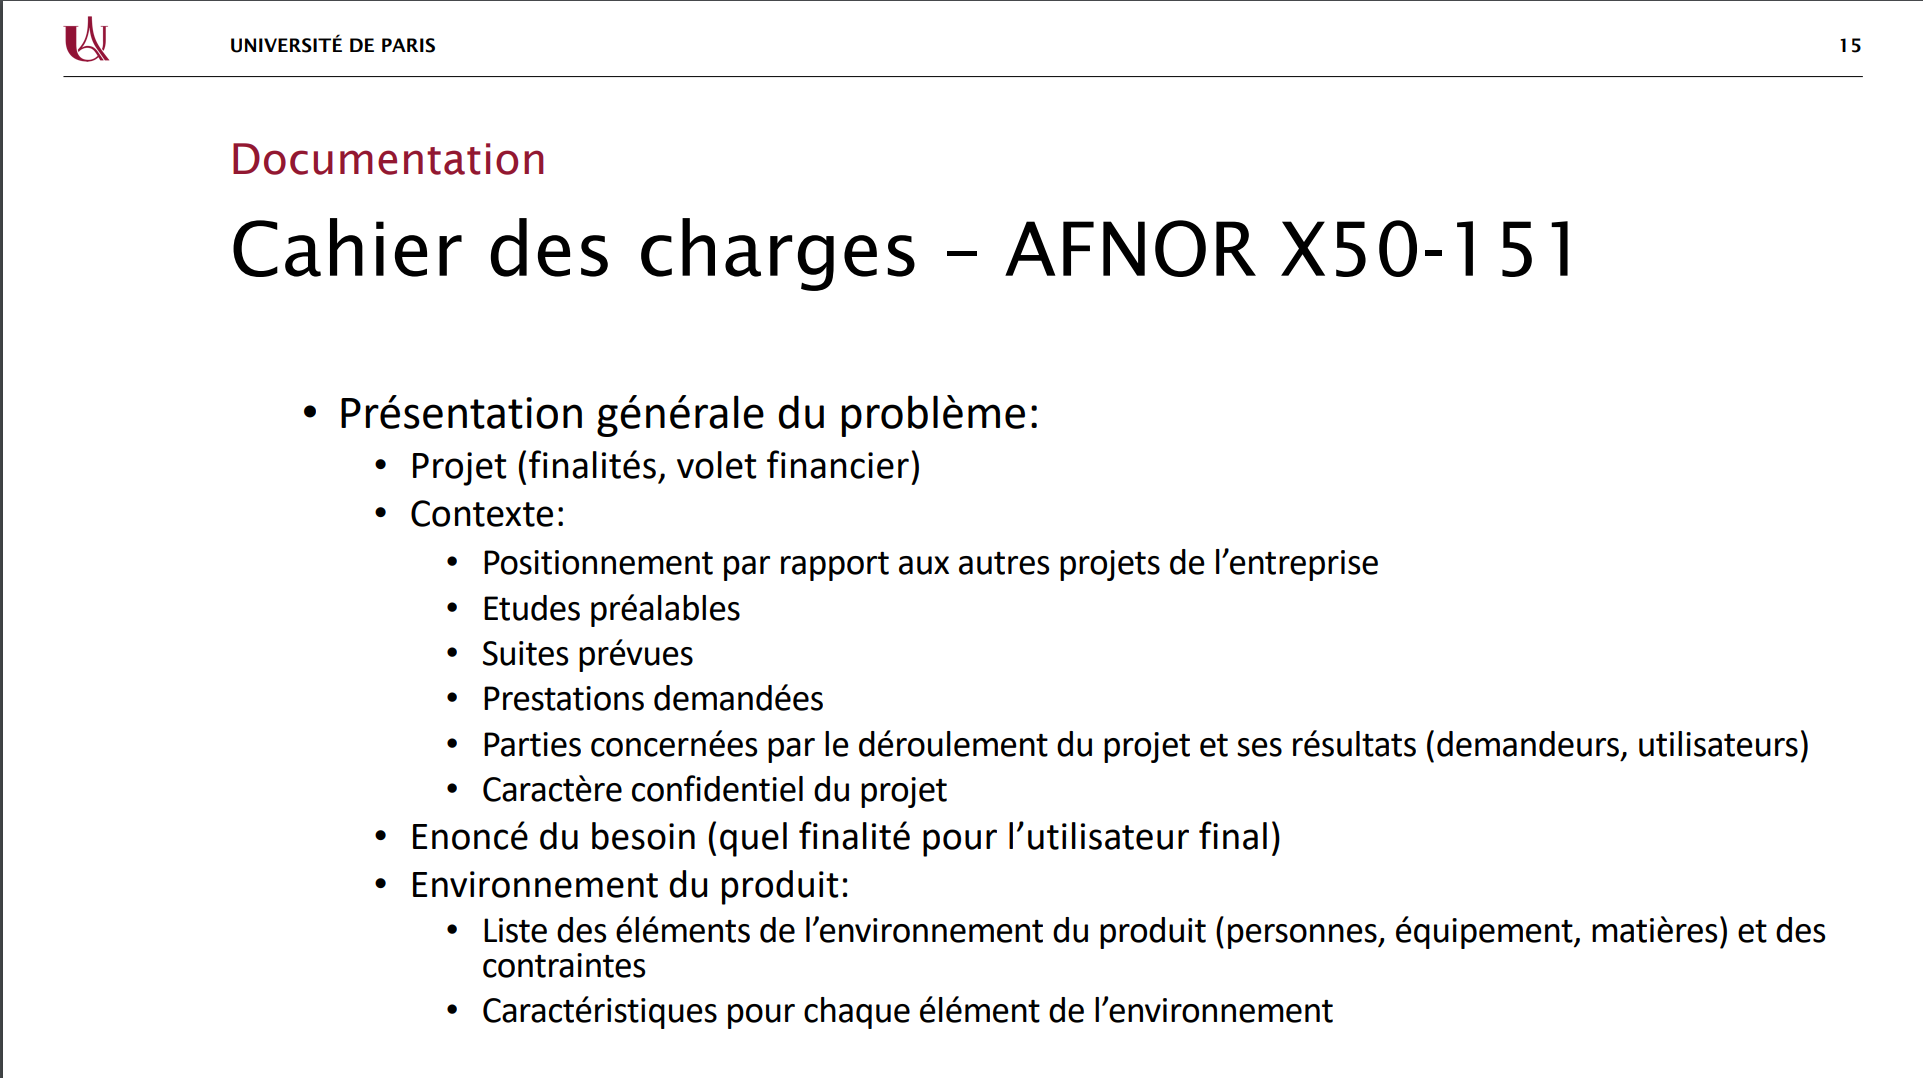
\includegraphics[scale=0.75]{Capture2.PNG}
	%\caption{Légende de l'image}
\end{figure}
\newpage
\begin{figure}[!hbtp]
	\centering
	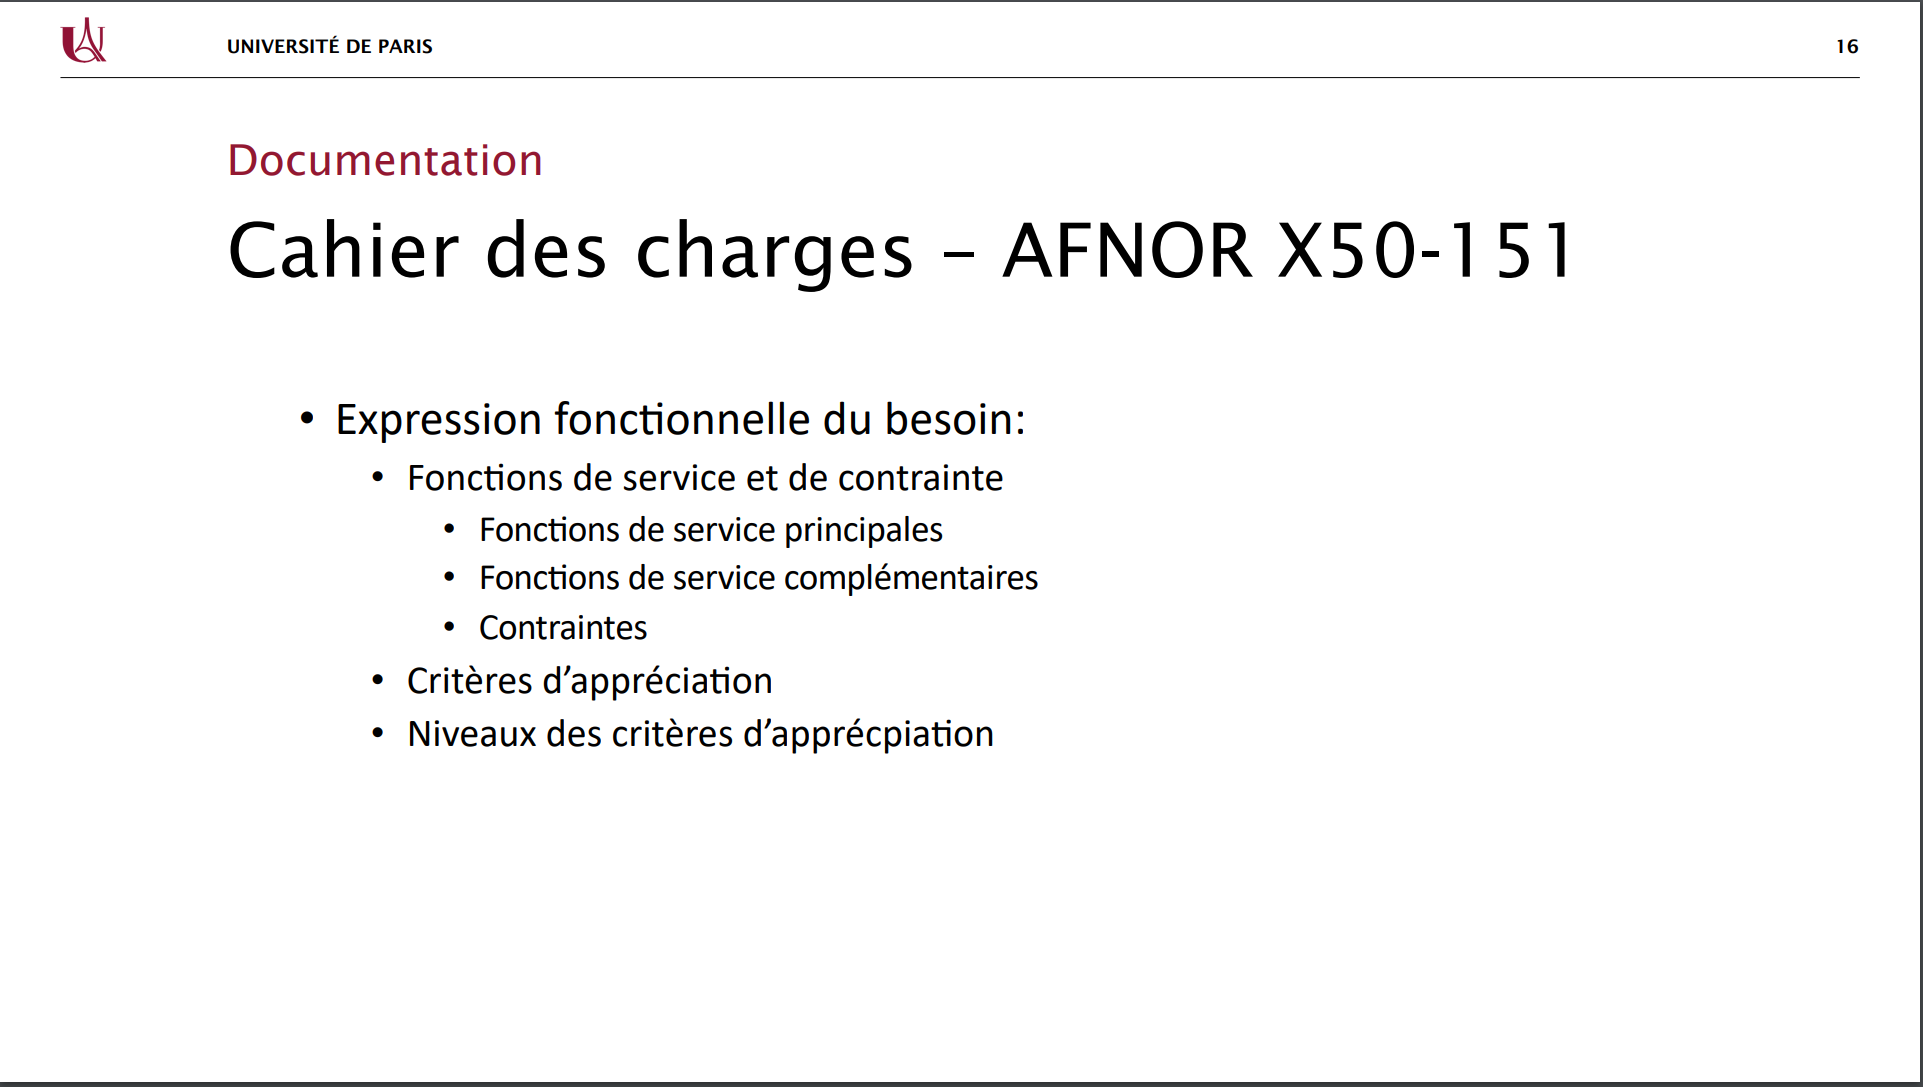
\includegraphics[scale=0.75]{Capture3.PNG}
	%\caption{Légende de l'image}
\end{figure}
\begin{figure}[!hbtp]
	\centering
	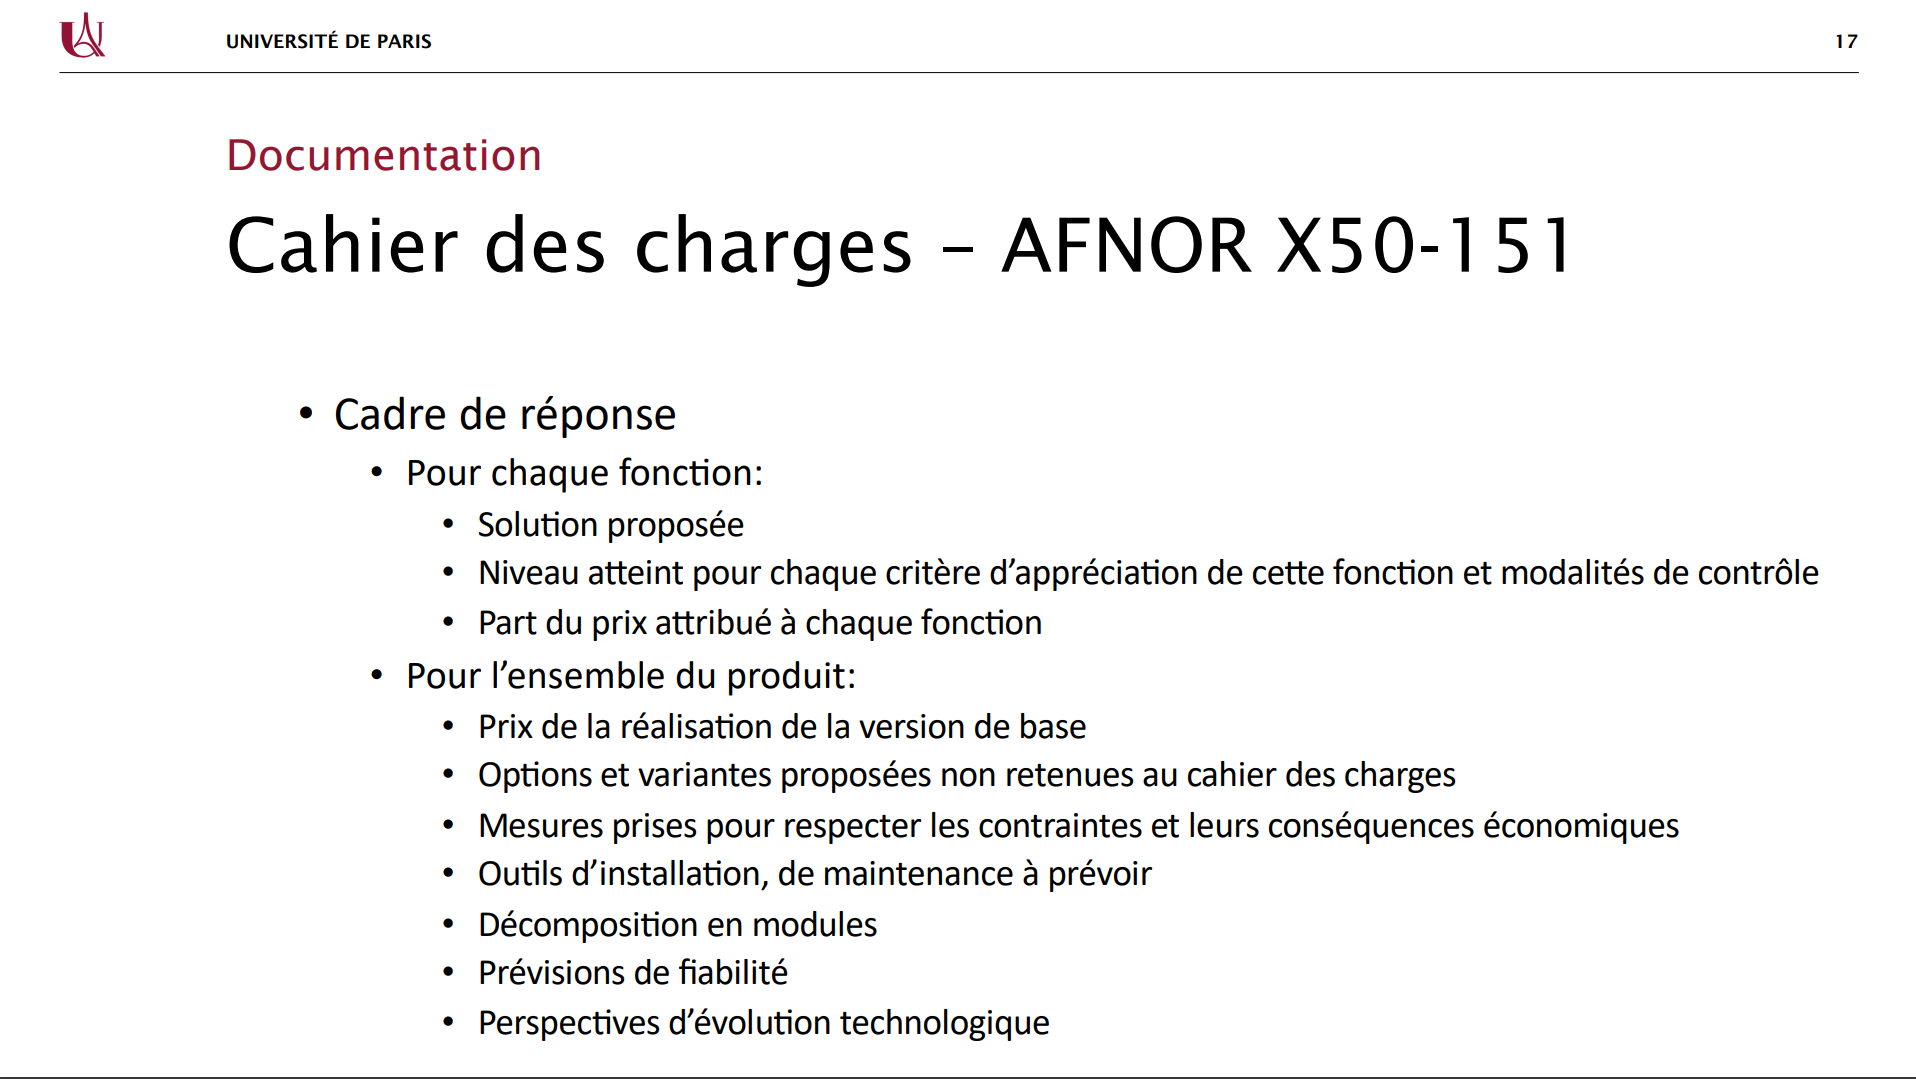
\includegraphics[scale=0.75]{Capture4.PNG}
	%\caption{Légende de l'image}
\end{figure}
\subsection{Plan de développement}
\begin{itemize}
	\item[* ] Définition : document qui présente la stratégie de développement
	\item[* ] Objectif : fournir une référence sur la planification et l'organisation de l'aménagement du territoire.
	développement du logiciel
\end{itemize}
\subsection{Plan de développement - sections}
\begin{itemize}
	\item[* ] Introduction :
	\begin{itemize}
		\item[* ] Objectifs du développement
		\item[* ] Méthodologie
		\item[* ] Documents connexes
		
	\end{itemize}
\item[* ] Organisation :
\begin{itemize}
	\item[* ] Description des tâches
	\item[* ] Description du personnel
\end{itemize}
\item[* ] Planification :
\begin{itemize}
	\item[* ] Cycle de vie du développement logiciel
	\item[* ] Chronologie
	\item[* ] Méthodes et choix technologiques
\end{itemize}
	\item[* ] Documentation :
	\begin{itemize}
		\item[* ] Quel document va soutenir le développement
		\item[* ] Quelle norme sera suivie
		\item[* ] Quels outils de gestion seront utilisés
		\item[* ] Qualité : quelle norme de qualité sera utilisée, comment allez-vous évaluer la qualité ?
	\end{itemize}
\end{itemize}
\subsection{Conception}
\begin{itemize}
	\item[* ] Définition : document qui présente les résultats de la phase de conception, avec une
	description complète et détaillée des composants du logiciel.
	\item[* ] Objectif : référence pour les développeurs et la direction.
\end{itemize}
\subsection{Conception - sections}
\newpage
	\begin{figure}[!hbtp]
	\centering
	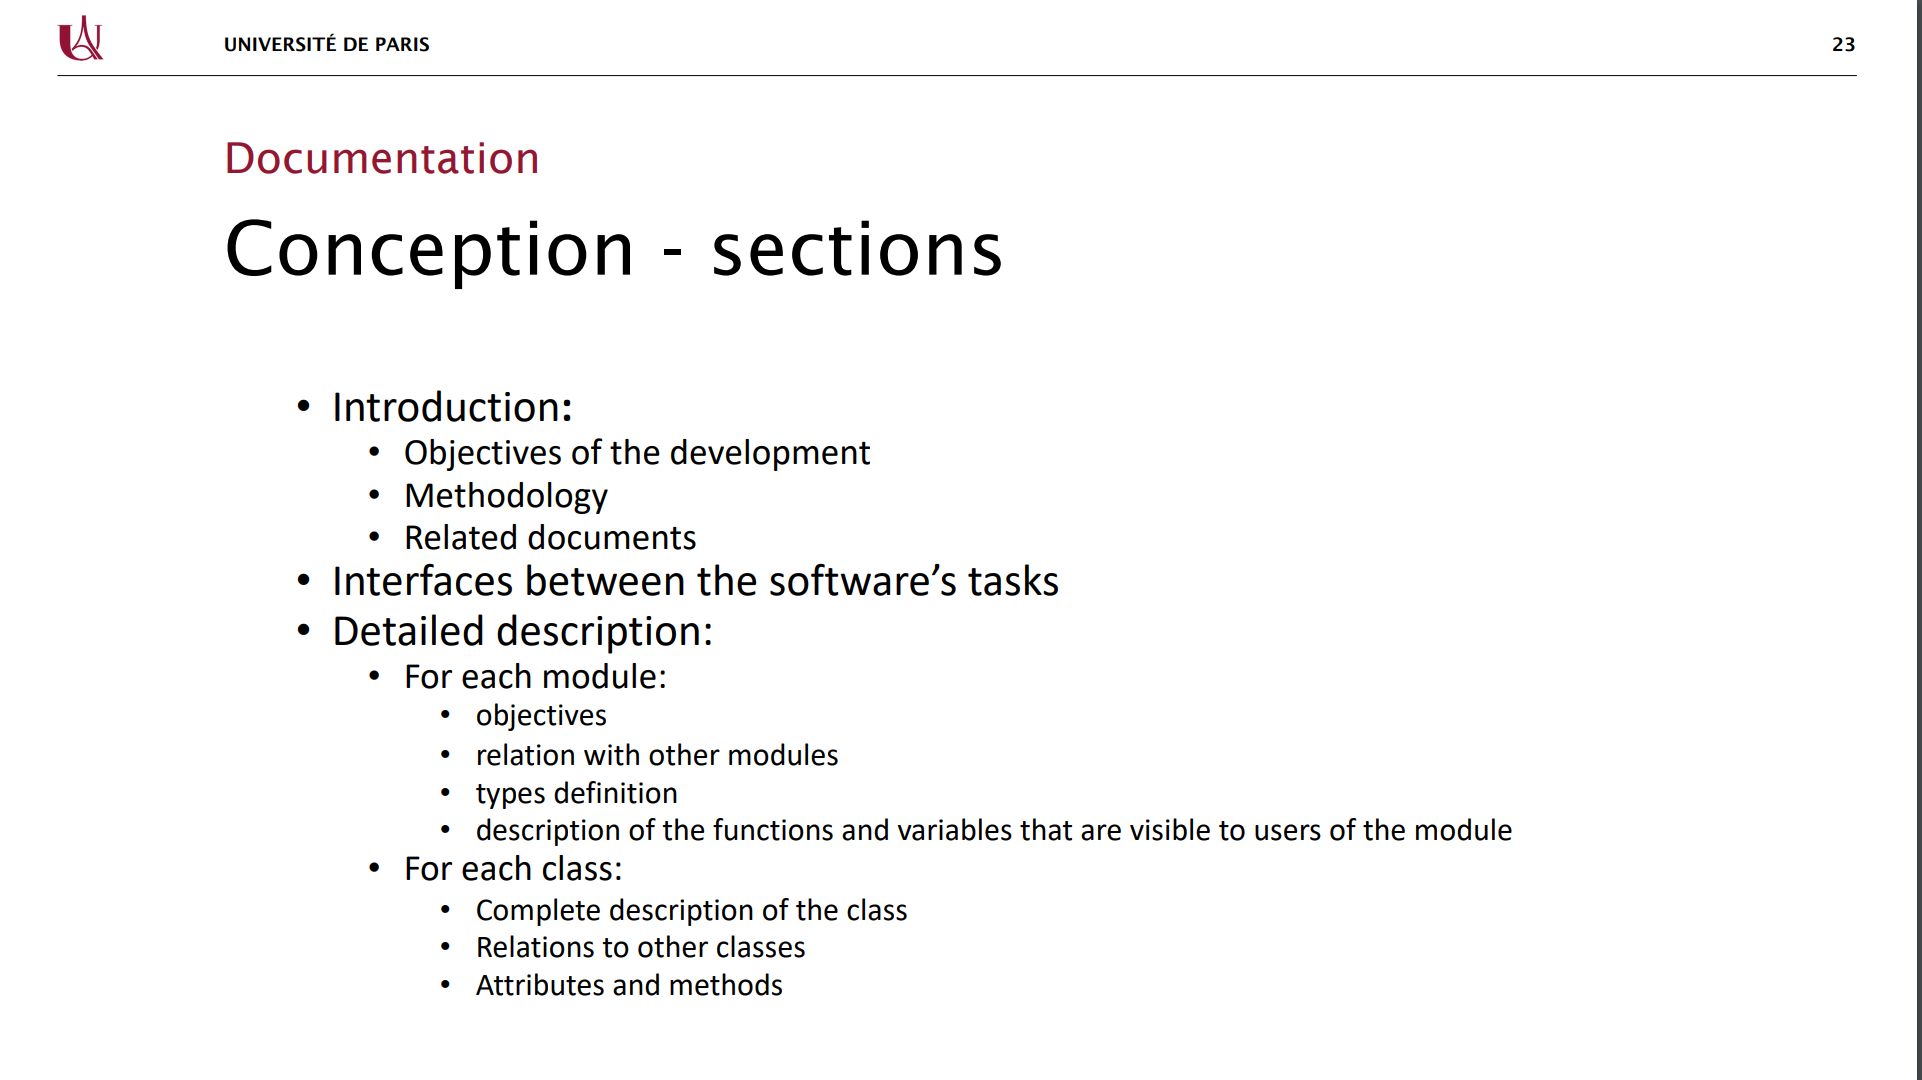
\includegraphics[scale=0.75]{Capture5.PNG}
	%\caption{Légende de l'image}
\end{figure}
\subsection{Plan de test}
\begin{itemize}
	\item[* ] Définition : décrit la procédure de test complète permettant de vérifier le
	logiciel dans son intégralité et chaque composant individuellement
	\item[* ] Objectif : décrire les tests unitaires (pour tester chaque composant) et les tests d'intégration (pour tester le logiciel complet) avant la phase d'implémentation.
\end{itemize}
\newpage
	\begin{figure}[!hbtp]
	\centering
	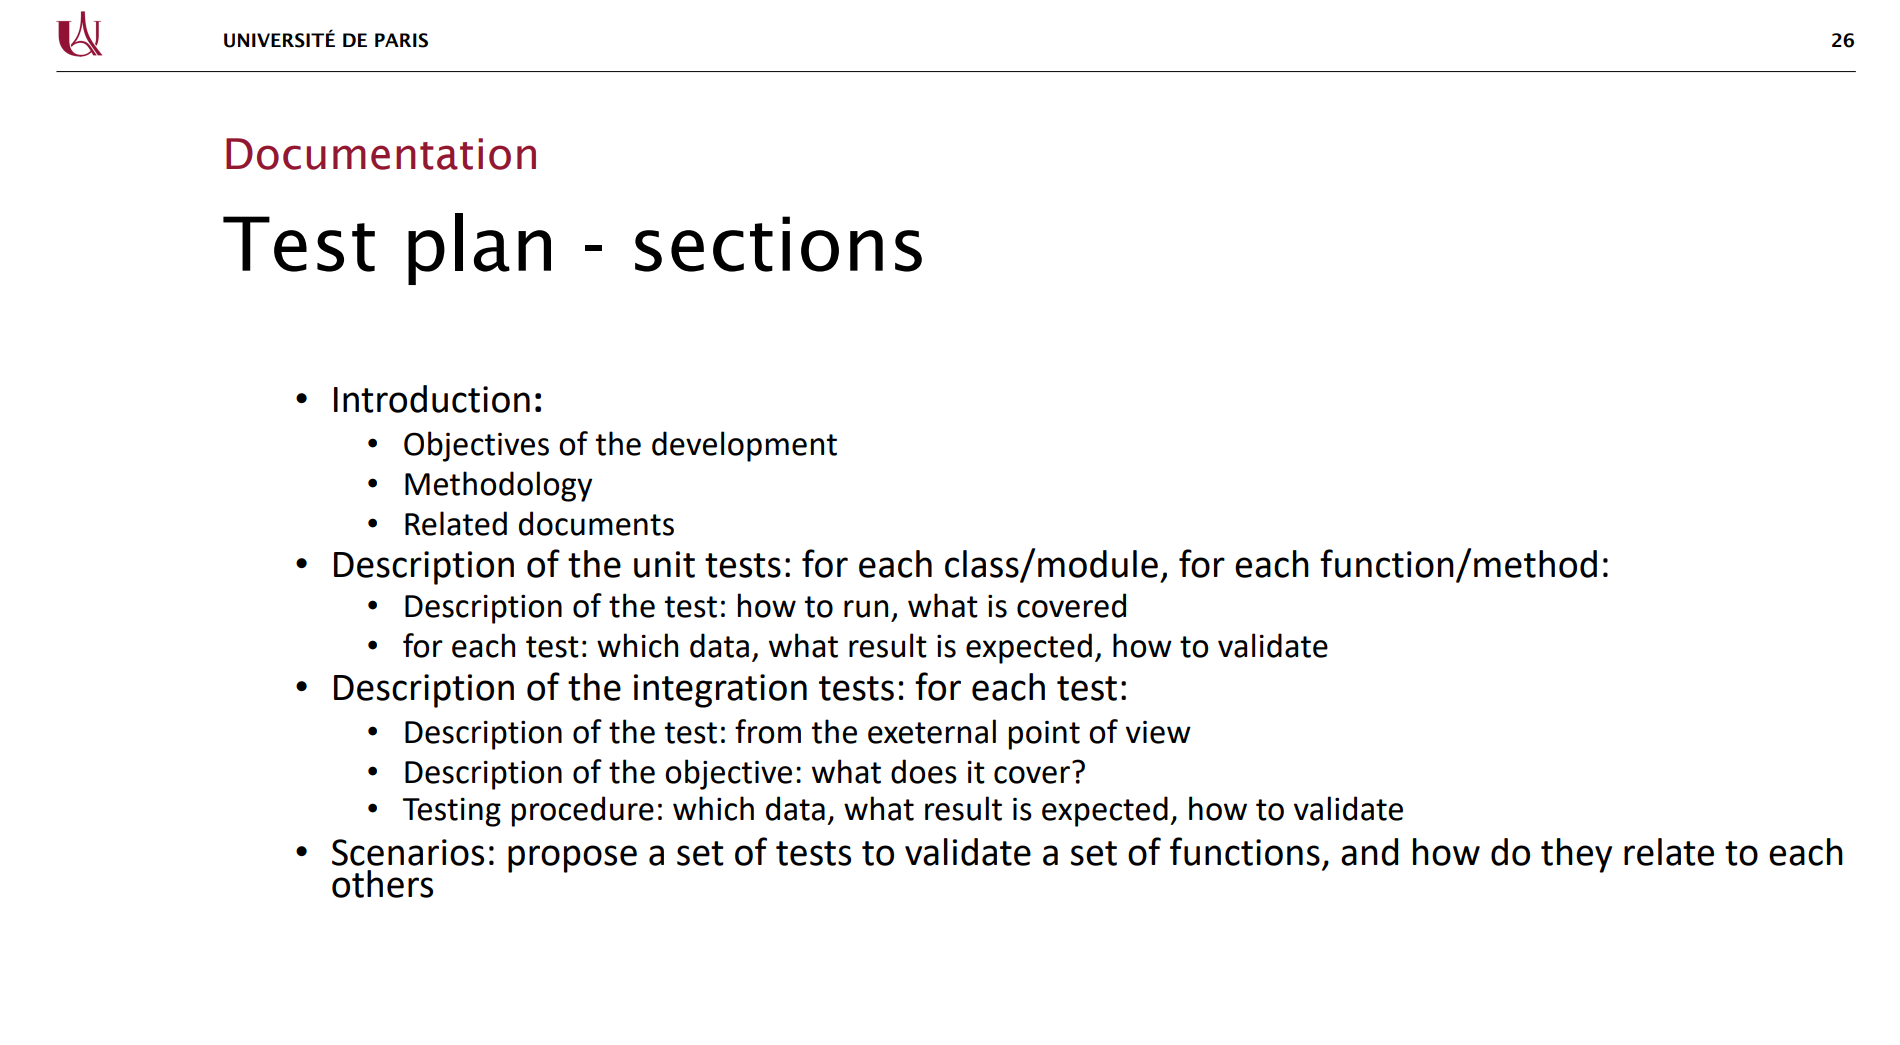
\includegraphics[scale=0.75]{Capture6.PNG}
	%\caption{Légende de l'image}
\end{figure}
\subsection{Acceptance plan (cahier de recette)}
\begin{itemize}
	\item[* ] Définition : décrit les différents aspects de la livraison de logiciels, notamment
	les tests d'acceptation
	\item[* ] Définition (tests d'acceptation) : Test formel par rapport aux besoins des utilisateurs,
	des utilisateurs, des exigences et des processus d'affaires, afin de déterminer si un
	système satisfait aux critères d'acceptation et pour permettre à l'utilisateur, aux clients ou à une autre entité autorisée de déterminer s'il faut accepter le système.
	\item[* ] Objectif : définir contractuellement la manière de valider que le logiciel répond aux besoins et exigences prédéfinis.
\end{itemize}
\newpage
	\begin{figure}[!hbtp]
	\centering
	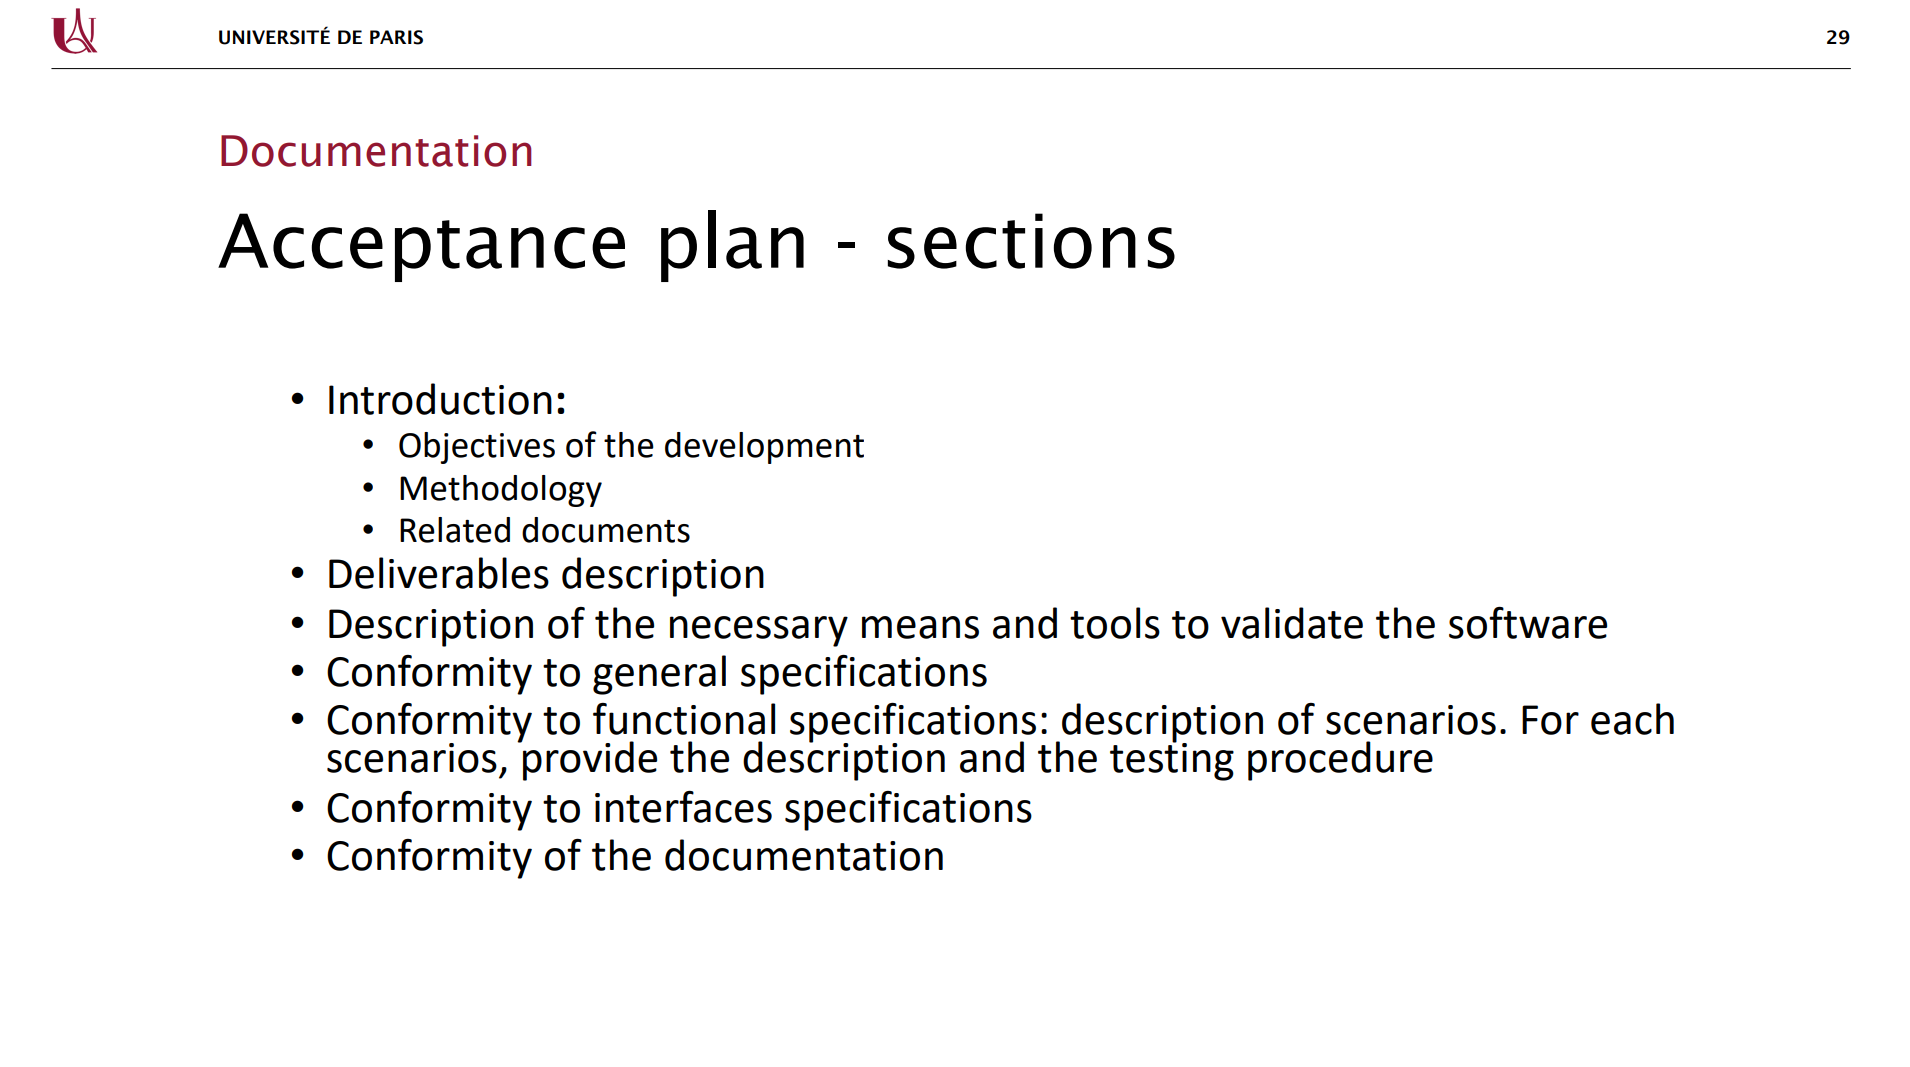
\includegraphics[scale=0.75]{Capture7.PNG}
	%\caption{Légende de l'image}
\end{figure}
\subsection{Manuel d'installation}
\begin{itemize}
	\item[* ] Définition : le manuel d'installation est un document qui rassemble toutes les
	procédures nécessaires pour installer le logiciel dans son environnement de production.
	\item[* ] Objectif : permettre à l'administrateur système d'installer et de configurer le logiciel sur le système d'information visé.
\end{itemize}
\subsection{Manuel d'installation - sections}
\begin{itemize}
	\item[* ] Installation du matériel : quel matériel doit être installé, quelle procédure
	sont nécessaires pour la production
	\item[* ] Configuration du système : quels paramètres doivent être appliqués pour correctement
	configurer le système
	\item[* ] Installation du logiciel : quelle est la procédure à suivre pour installer le logiciel sur le
	système
	\item[* ] Configuration du logiciel : quels sont les paramètres à appliquer pour 
	configurer le logiciel
	\item[* ] Données : quelles sont les procédures à suivre pour configurer les données du logiciel ?
	\item[* ] Autres informations : conflits éventuels avec d'autres parties du système,
	mode de maintenance
\end{itemize}
\subsection{Manuel d'utilisation}
\begin{itemize}
	\item[* ] Définition : le manuel d'utilisation est un document décrivant les fonctionnalités du
	le logiciel et les informations sur la façon de les utiliser.
	\item[* ] Objectif : permettre à l'utilisateur final du logiciel d'utiliser toutes les fonctionnalités du logiciel.

\end{itemize}
\subsection{Manuel de l'utilisateur - sections}
\begin{itemize}
	\item[* ] Opérations de base : comment utiliser le logiciel pour utiliser les différentes fonctions
	fournies par
	\item[* ] Dépannage : description des exceptions/codes d'erreur, liste des problèmes éventuels et
	problèmes possibles et comment les résoudre
\end{itemize}
\subsection{Conseils généraux sur la façon de rédiger des documents}
	\begin{figure}[!hbtp]
	\centering
	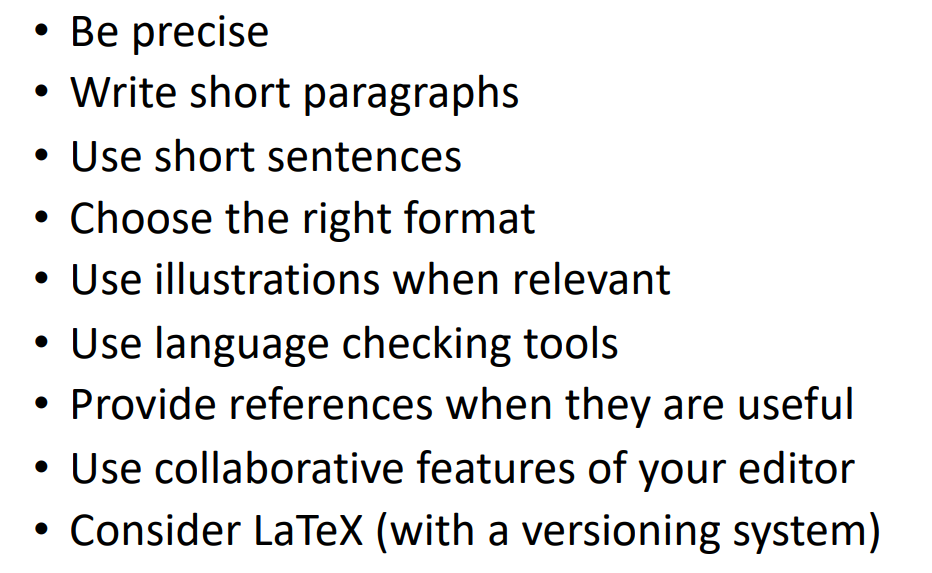
\includegraphics[scale=0.75]{Capture8.PNG}
	%\caption{Légende de l'image}
\end{figure}
\subsection{Conclusion}
\begin{figure}[!hbtp]
	\centering
	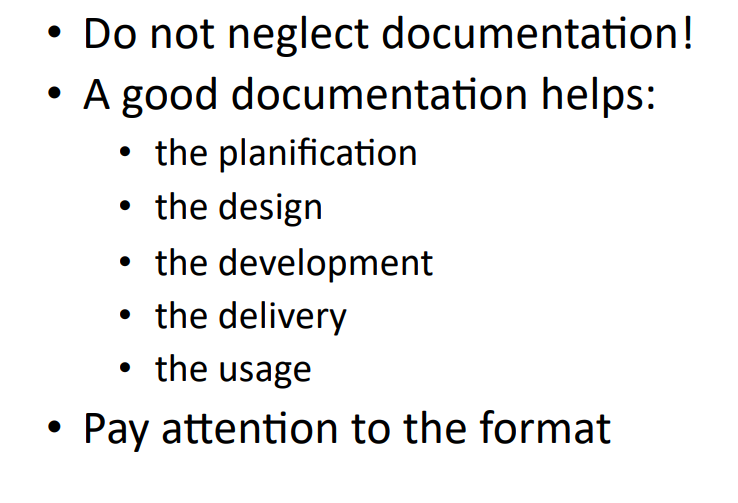
\includegraphics[scale=0.75]{Capture9.PNG}
	%\caption{Légende de l'image}
\end{figure}
\section{Génie logiciel}
\subsection{Développement logiciel agile}
\begin{figure}[!hbtp]
	\centering
	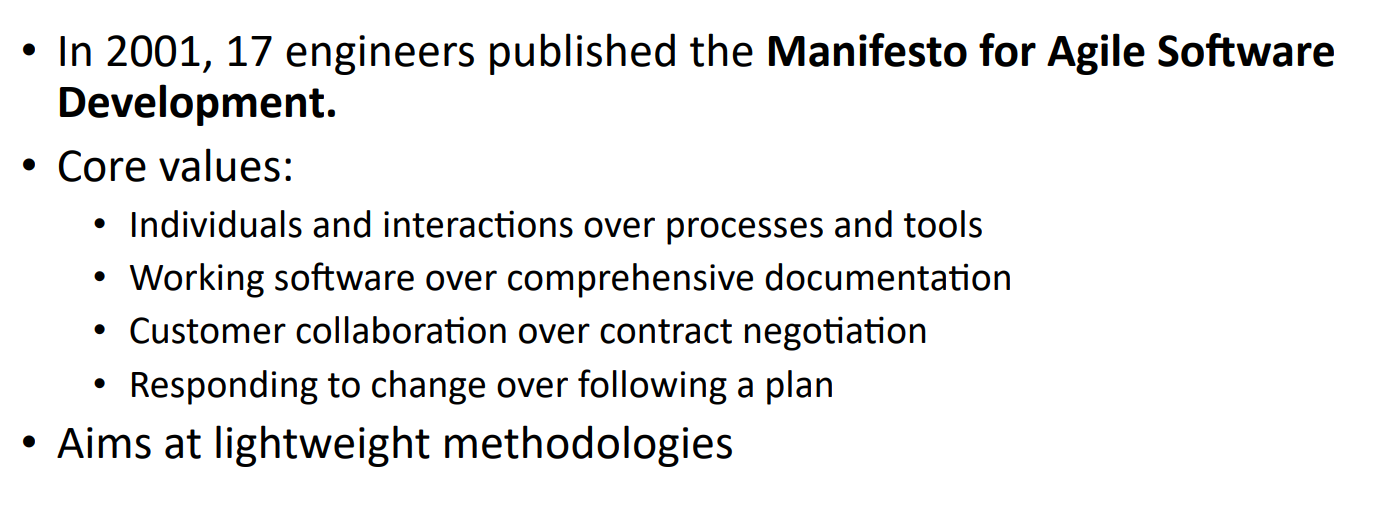
\includegraphics[scale=0.75]{Capture10.PNG}
	%\caption{Légende de l'image}
\end{figure}
Le manifeste présente 12 principes : \\
- Notre priorité absolue est de satisfaire le client par la livraison rapide et continue de logiciels de qualité.\\
- Accueillir l'évolution des besoins, même à un stade avancé du développement. Les processus agiles exploitent le changement pour l'avantage concurrentiel du client.\\
- Livrer fréquemment des logiciels fonctionnels, de quelques semaines à quelques mois, avec une préférence pour les délais les plus courts.\\
- Les responsables commerciaux et les développeurs doivent collaborer quotidiennement tout au long du projet.\\
- Construisez des projets autour de personnes motivées. Donnez-leur l'environnement et le soutien dont ils ont besoin, et faites-leur confiance
pour faire le travail.\\
- La méthode la plus efficace pour transmettre des informations à une équipe de développement et au sein de celle-ci est la conversation en face à face.\\
- Le logiciel fonctionnel est la principale mesure du progrès.\\
- Les processus agiles favorisent le développement durable. Les commanditaires, les développeurs et les utilisateurs doivent être en mesure de
maintenir indéfiniment un rythme constant.\\
- Une attention constante à l'excellence technique et à une bonne conception renforce l'agilité.\\
- La simplicité - l'art de maximiser la quantité de travail non effectué - est essentielle.\\
- Les meilleures architectures, exigences et conceptions émergent d'équipes auto-organisées.\\
- À intervalles réguliers, l'équipe réfléchit à la manière de devenir plus efficace, puis adapte et ajuste son comportement en conséquence.
\end{document}